% Layer-2 technical report (CLAUDE.md §8 item 127). Build: see build.sh in this folder.
\documentclass[conference]{IEEEtran}
\usepackage{amsmath,amssymb}
\usepackage{graphicx}
\usepackage{booktabs}
\usepackage{algorithm}
\usepackage[noend]{algpseudocode}
\usepackage{cite}
\usepackage{xcolor}
\usepackage{siunitx}
\graphicspath{{figs/}}
\algrenewcommand\algorithmicrequire{\textbf{Input:}}
\algrenewcommand\algorithmicensure{\textbf{Output:}}
\algrenewcommand\algorithmiccomment[1]{\hfill{\color{black!60}$\triangleright$ #1}}
\newcommand{\CapC}{\mathrm{Cap}}
\newcommand{\CH}{\mathrm{CH}}

\begin{document}

\title{Flight-First Cluster Design for Single-Pass\\Fixed-Wing UAV Query Delivery}
\author{\IEEEauthorblockN{Technical Report --- Layer 2 of Phase 1 (flight line and clustering)}
\IEEEauthorblockA{Version 22 Oct.\ 2026. All numbers are exploratory (one ns-3 pass per cluster; $N<120$).}}
\maketitle

\begin{abstract}
A fixed-wing UAV delivers a search query (a clue set of $Q$ packets) to a network of IoT cameras by flying over each
cluster \emph{once} and broadcasting one IEEE~802.15.4 packet every \SI{0.5}{m}. Because every packet is emitted at a
known point of the path, the geometry of the flight line and of the clusters fixes how much data each cluster
receives, which cells hear it in long contiguous runs, and how much ground cooperation (Layer~3, River) is left to do.
This report presents the two Layer-2 procedures we built on this observation: \textsc{Chord}, which flies the longest
chord through the cluster head of a given cluster, and \textsc{Meander}, which partitions the land into
River-wide lanes along its geodesic spine and flies a curvature-bounded path through each cluster head. \textsc{Chord}
raises the data per pass by up to 88\,\%; \textsc{Meander} raises the share of cells inside the River band from
55--57\,\% to 83--90\,\%. At mission level, however, \textsc{Meander} does not yet beat \textsc{Chord} on existing
clusters: it creates 20--65\,\% more clusters and a longer tour. We report why, the cluster shape at which River
saturates (lanes 8--10 cells wide, 2--3\,km long), and the fair comparison that remains to be run.
\end{abstract}

\section{Core Idea}
Phase~1 of the mission has three layers: what a camera needs to recognise the target (Layer~1), how the UAV delivers
it (Layer~2) and how the ground network completes the delivery (Layer~3). The UAV is fixed-wing: it cannot hover and
passes over each cluster once, at \SI{50}{m/s} and \SI{100}{m}. Cells near the path hear long runs of packets; cells
far from it hear scattered packets that cannot be assembled into files. Layer~3 (River) then moves the missing
packets to a few \emph{critical cells} that will run the matching.

\textbf{Key observation: in a single-pass broadcast, the geometry is the schedule.} Packet $s$ is sent at
$\gamma(d_s)$, $d_s=d_0+s\Delta$, $\Delta=\SI{0.5}{m}$, and $\gamma$ is planned by the base station (BS). Hence,
before the flight,
\begin{itemize}
\item the in-cluster length of $\gamma_k$ fixes the data $D_k$ that cluster $k$ receives;
\item the cells within the River half-width $\omega$ of $\gamma_k$ are those that hold long contiguous runs;
\item the number of clusters fixes the number of entries, exits and turns of the tour, and the number of cluster heads
(each one a critical cell).
\end{itemize}
Layer~2 should therefore design the flight lines and the clusters \emph{together}. We pursue three principles:
\textbf{(P1)} fly the longest chord through each cluster head; \textbf{(P2)} choose the flight lines first and cut
the clusters along them (flight-first partitioning); \textbf{(P3)} size the clusters to the clue set and to the
point where River saturates.

\section{System Model and Layer-2 Problem}
\textbf{Domain.} The land is a set $\mathcal H$ of hexagonal cells of radius $R=\SI{100}{m}$ (width
$w=\sqrt3R\approx\SI{173}{m}$), about 21 nodes per cell. Lakes are holes: no nodes, but the UAV may fly over them.
$d(a,b)$ is the geodesic distance over land cells. Each cell has a cell leader (CL), its strongest node.

\textbf{UAV.} Speed $v=\SI{50}{m/s}$, minimum turn radius $\rho=\SI{255}{m}$ (\ang{45} bank). One packet of
\SI{99}{B} payload every \SI{10}{ms}; the clue set has $Q=4036$ packets, about \SI{2.0}{km} of flight. Links between
clusters are Dubins paths~\cite{dubins1957}.

\textbf{Outputs of Layer~2.} Clusters $\{\mathcal C_k\}$ that partition $\mathcal H$, each connected with
$|\mathcal C_k|\le\CapC$ ($\CapC=80$); a cluster head $\CH_k$, the strongest node at least \SI{300}{m} from the cluster
edge; a flight path $\gamma_k$ through $\CH_k$ with curvature $\kappa\le1/\rho$ and straight leads of length $\rho$
outside $\mathcal C_k$; and a visiting order $\pi$.

\textbf{Metrics.} $D_k=\{s:\gamma(d_s)\in\mathcal C_k\}$; River coverage
$\varrho=\sum_k|\{h\in\mathcal C_k:\mathrm{dist}(z_h,\gamma_k)\le\omega\}|/|\mathcal H|$ with $\omega=1.75w\approx
\SI{303}{m}$; tour time $T_1$; and the mission time $T^\star$, at which the second UAV team has verified the
top-scored cell $c^\star$. $T^\star$ couples all layers, so Layer~2 is designed on three proxies: $|D_k|\ge Q$
(the clue set fits), large $\varrho$ (short River), and small $T_1$ (few clusters, short links).

\section{Procedure 1: Longest Chord Through the Cluster Head}
For an existing partition (capacitated geodesic $k$-medoids~\cite{kaufman1990}), \textsc{Chord}
(Alg.~\ref{alg:chord}) scans the straight lines through $\CH_k$ and flies the one with the longest in-cluster
length. Entry and exit are the farthest points of the line still in the cluster, so the UAV crosses lakes and
neighbour clusters in between (soft obstacles). The visiting order minimises the time at which every critical cell
holds its data, solved exactly by Held--Karp~\cite{heldkarp1962}.

\begin{algorithm}[t]
\caption{\textsc{Chord}: flight line of one cluster}\label{alg:chord}
\small
\begin{algorithmic}[1]
\Require cluster $\mathcal C$, its nodes, radius $\rho$, steps $\delta\theta=\ang{2}$, $\delta t=\SI{5}{m}$
\Ensure $\CH$, entry $p_\mathrm{in}$, exit $p_\mathrm{out}$, path $\gamma$
\For{margin $m\in(300,200,100,0)$\,m}
  \State $\CH\gets$ strongest node with edge distance $\ge m$; \textbf{if} found \textbf{break}
\EndFor
\For{$\theta\in\{0,\delta\theta,\dots,\ang{180}-\delta\theta\}$} \Comment{$\theta$, $\theta+\pi$: one line}
  \State $L(\theta)\gets\delta t\cdot|\{t\in\delta t\mathbb Z:|t|\le\SI{8}{km},\ \mathrm{cell}(\CH+t\,u_\theta)\in\mathcal C\}|$
\EndFor
\For{$\theta$ in decreasing order of $L(\theta)$}
  \State $p_\mathrm{in},p_\mathrm{out}\gets$ farthest points of the line in $\mathcal C$, one on each side of $\CH$
  \State $\gamma\gets$ shortest Dubins path $p_\mathrm{in}\to\CH\to p_\mathrm{out}$ (radius $\rho$) whose end
         headings cross the edge and whose leads of length $\rho$ lie outside $\mathcal C$
  \State \textbf{if} $\gamma\neq\emptyset$ \textbf{return} $(\CH,p_\mathrm{in},p_\mathrm{out},\gamma)$
\EndFor
\end{algorithmic}
\end{algorithm}

\begin{figure}[t]
\centering
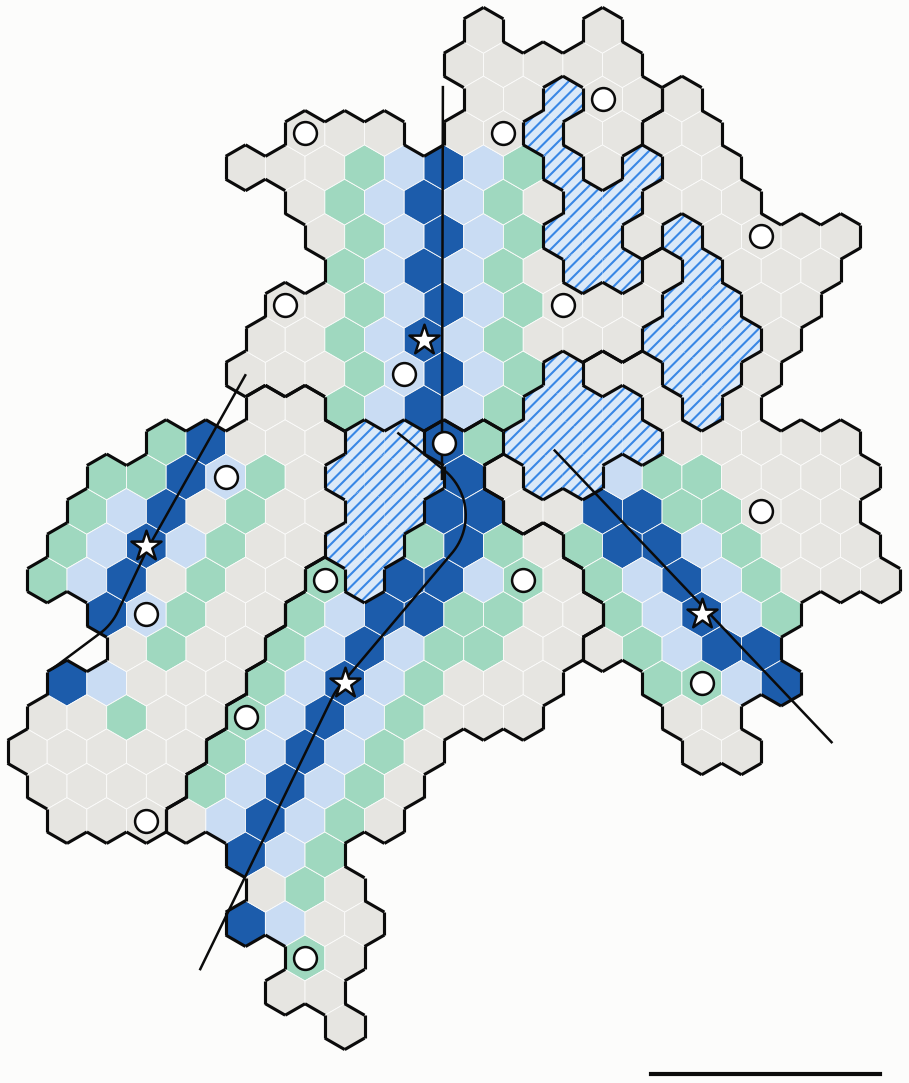
\includegraphics[width=0.48\columnwidth]{chord-before}\hfill
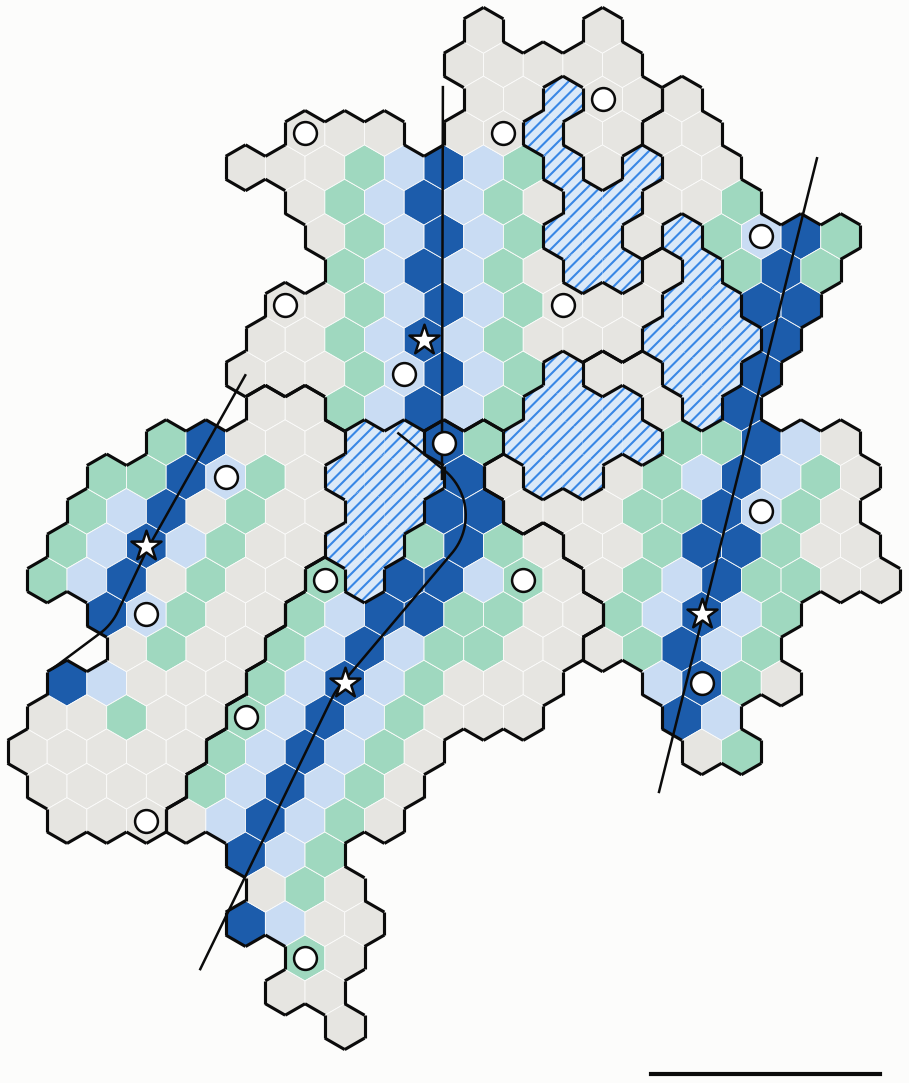
\includegraphics[width=0.48\columnwidth]{chord-after}\\[-1pt]
\makebox[0.48\columnwidth]{\footnotesize(a)}\hfill\makebox[0.48\columnwidth]{\footnotesize(b)}
\caption{\textsc{Chord} on a four-cluster map (bar: \SI{1}{km}). Dark blue: Axe (cells under the path); light
blue: River; green: Bank; star: $\CH$; circle: other critical cell; hatched: lake. (a)~Lines through $\CH$ from a
random edge point. (b)~The east cluster now flies its longest chord, across the lake: \SI{1.25}{km}~$\to$
\SI{2.34}{km} in the cluster, $|D|$ 2494~$\to$ 4685 packets (+88\,\%).}
\label{fig:chord}
\end{figure}

On the four clusters of Fig.~\ref{fig:chord}, the longest chord adds 61, 5, 88 and 79\,\% of in-cluster length. On
all 200 clusters of our 40 evaluation maps, the head margin had to drop to \SI{200}{m} for 14 thin clusters, and the
longest chord was always flyable: the loop of lines 5--8 never needed a second direction.

\section{Procedure 2: Flight-First Partitioning (\textsc{Meander})}
\textsc{Chord} keeps clusters that were cut without regard to the flight: a compact cluster has only about half of its
cells within $\omega$ of any single line. \textsc{Meander} (Alg.~\ref{alg:meander}) reverses the order. It first lays
out lanes as wide as the River, following the shape of the land, and then cuts each lane into clusters along its
length. The steps are shown in Fig.~\ref{fig:steps}.

\begin{figure*}[t]
\centering
\setlength{\tabcolsep}{1pt}
\begin{tabular}{cccccccc}
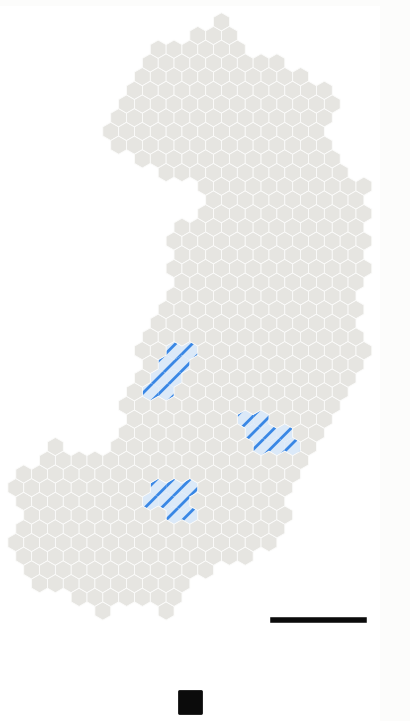
\includegraphics[width=0.118\textwidth]{meander-a}&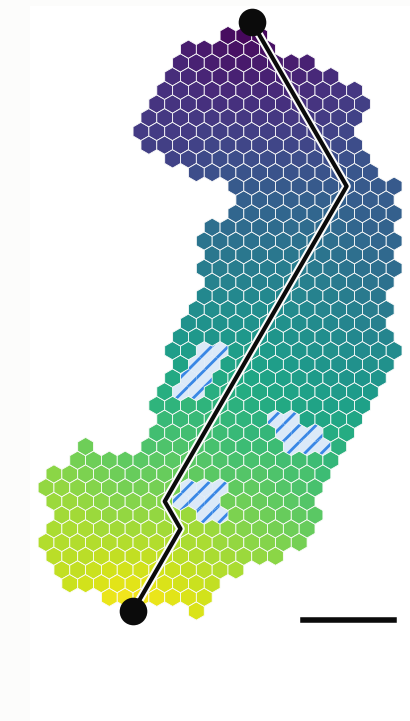
\includegraphics[width=0.118\textwidth]{meander-b}&
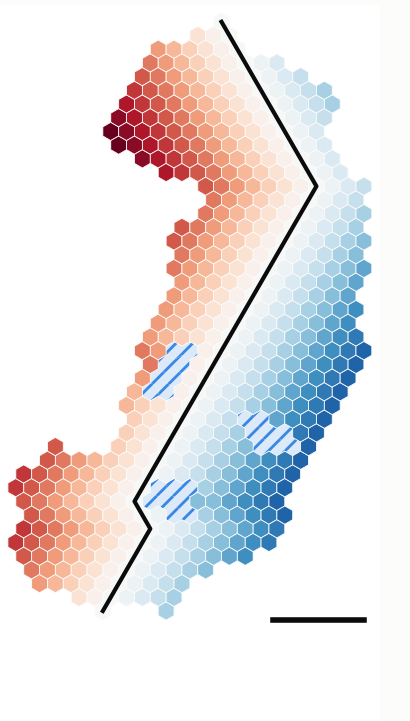
\includegraphics[width=0.118\textwidth]{meander-c}&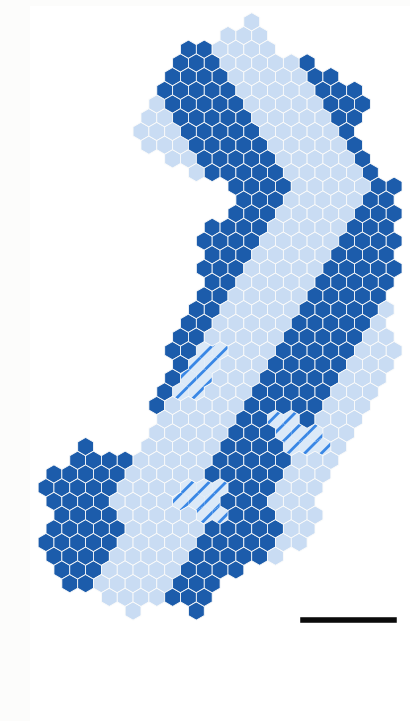
\includegraphics[width=0.118\textwidth]{meander-d}&
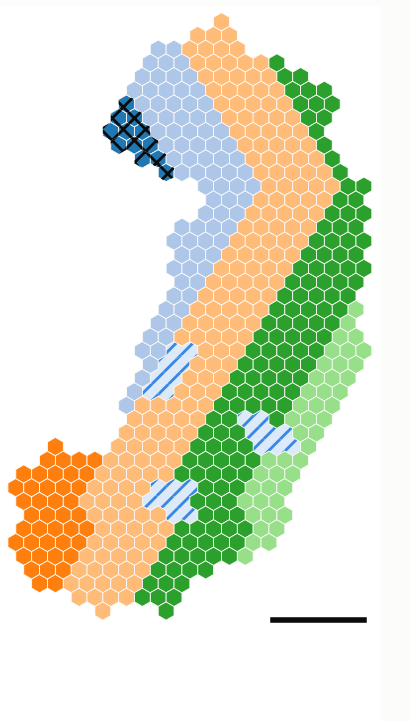
\includegraphics[width=0.118\textwidth]{meander-e}&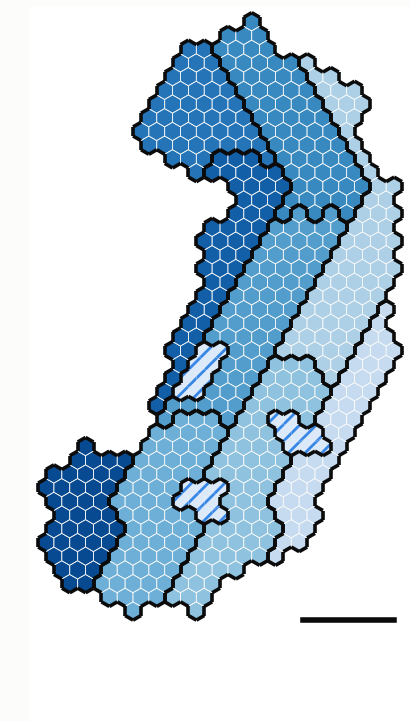
\includegraphics[width=0.118\textwidth]{meander-f}&
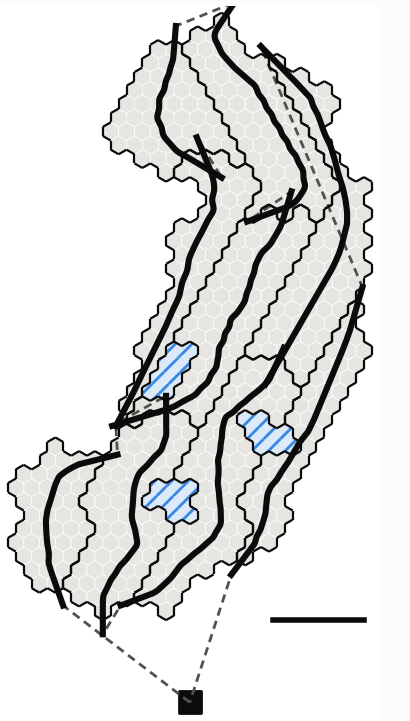
\includegraphics[width=0.118\textwidth]{meander-g}&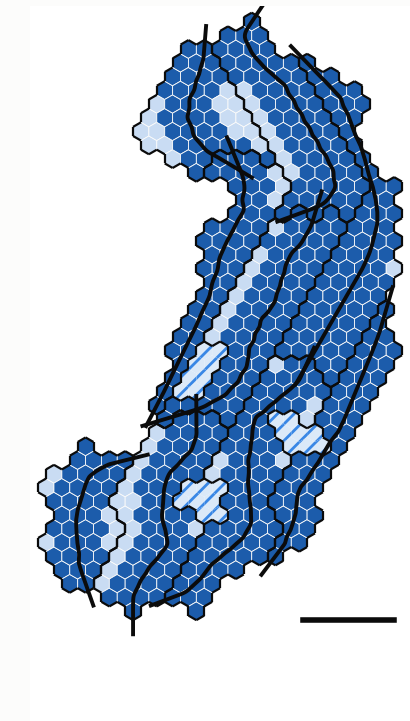
\includegraphics[width=0.118\textwidth]{meander-h}\\
\footnotesize(a)&\footnotesize(b)&\footnotesize(c)&\footnotesize(d)&\footnotesize(e)&\footnotesize(f)&
\footnotesize(g)&\footnotesize(h)
\end{tabular}
\caption{\textsc{Meander} step by step on a curved domain (\ang{220} bend, about \SI{1}{km} wide, 480 cells, three
lakes; bar: \SI{1}{km}). (a)~Land, lakes (hatched) and BS (square). (b)~Spine $A\to B$ (geodesic diameter) and
along-coordinate $s$, purple at $A$ to yellow at $B$. (c)~Across-coordinate $n$: signed geodesic distance to the
spine, red on one side, blue on the other. (d)~Lanes of width $Lw$, alternating shades. (e)~Lane pieces; the
hatched fragments are merged into a neighbour. (f)~Clusters, darker = visited earlier. (g)~Smoothed flight
curves (bold) and the tour (dashed). (h)~River coverage: dark = within $\omega$ of the own cluster's path
(88.5\,\% of cells).}
\label{fig:steps}
\end{figure*}

\textbf{Geodesic coordinates (lines 1--4).} The spine is the shortest land path between the two ends of the
geodesic diameter, found with two Dijkstra sweeps~\cite{dijkstra1959}. The coordinate $s(h)=(d(A,h)-d(B,h))/2$ runs
along the land and bends round lakes; $n(h)$ is the signed geodesic distance to the spine, its side taken from the
spine's local tangent where the wavefront leaves it. Iso-lines of $n$ follow the bends where straight
lanes~\cite{huang2001,choset2000} would cut across them.

\textbf{Lanes and clusters (lines 5--10).} Lanes are strips of $n$ of width $Lw$. Three offsets are tried and the one
with the fewest clusters plus fragments is kept. Lakes split lanes into pieces; pieces smaller than $f\cdot\CapC$
join the neighbour with the longest shared border. Each piece is cut along $s$ into $\lceil|P|/\CapC\rceil$ equal
consecutive chunks, so every cluster is long and narrow and its path runs along it.

\begin{algorithm}[t]
\caption{\textsc{Meander}: flight-first partitioning (BS)}\label{alg:meander}
\small
\begin{algorithmic}[1]
\Require land cells $\mathcal H$ (lakes are holes), $\CapC$, lane width $L$, fragment ratio $f$, radius $\rho$
\Ensure clusters $\{\mathcal C_k\}$, paths $\{\gamma_k\}$, order $\pi$
\For{each connected land piece}
  \State $A\gets\arg\max_h d(h_0,h)$;\ $B\gets\arg\max_h d(A,h)$;\ Spine $\gets$ path $A\to B$
  \State $s(h)\gets\big(d(A,h)-d(B,h)\big)/2$ \Comment{along}
  \State $n(h)\gets$ signed geodesic distance to Spine \Comment{across}
\EndFor
\State $o^\star\gets\arg\min_{o\in\{0,\frac13,\frac23\}}\ \#\text{clusters}+\#\text{fragments}$ of
       $\mathrm{lane}_o(h)=\lfloor n(h)/(Lw)+o\rfloor$
\State $\mathcal P\gets$ connected pieces of the lanes $\mathrm{lane}_{o^\star}$
\While{some $P\in\mathcal P$ with $|P|<f\CapC$ touches another piece}
  \State merge the smallest such $P$ into its longest-border neighbour
\EndWhile
\For{each $P\in\mathcal P$}
  \State sort $P$ by $s$; cut into $\lceil|P|/\CapC\rceil$ equal consecutive chunks
\EndFor
\For{each cluster $\mathcal C_k$}
  \State $\CH_k\gets$ as in Alg.~\ref{alg:chord}, line~2;\ $\gamma_k\gets\textsc{Bend}(\mathcal C_k,s,\CH_k,\rho)$
\EndFor
\State $\pi\gets$ shortest of 4 boustrophedon tours (lane by lane, alternating)
\end{algorithmic}
\end{algorithm}

\textbf{Curvature-bounded path through the head (Alg.~\ref{alg:bend}).} The centre curve of a lane cluster is
smoothed by a Laplacian iteration until $\kappa\le1/\rho$. It must also pass through $\CH_k$, which hears the UAV
directly and is always critical. \textsc{Bend} adds a Gaussian bump $v\,e^{-(s-s^\star)^2/2\sigma^2}$ towards the
head. Its peak curvature is about $|v|/\sigma^2$, so $\sigma=\sqrt{2|v|\rho}$ keeps the bump alone within
$1/(2\rho)$; the curve is then smoothed again with the head pinned (Fig.~\ref{fig:bend}). All 28 clusters of three
mission maps were bent successfully; one needed $\sigma$ tripled. On a curved Axe, Layer~3 builds the Banks along the
\emph{local} normal of $\gamma$: at a \ang{70} exit angle this raises River coverage from 0.78 to 0.98 and Bank
offset from the path from $0.63\omega$ to $0.88\omega$ (ideal: $\omega$), with unchanged ns-3 completion times
(9.0 vs.\ \SI{9.1}{s} on average).

\begin{algorithm}[t]
\caption{\textsc{Bend}: path of a lane cluster through its head}\label{alg:bend}
\small
\begin{algorithmic}[1]
\Require cluster $\mathcal C$, coordinate $s$, head $\CH$, radius $\rho$
\State $P\gets$ mean cell centre per $w/2$-bin of $s$; moving average over 7 bins
\State \textsc{Smooth}($P$): $P_i\gets P_i+\frac14(P_{i-1}+P_{i+1}-2P_i)$ until $\max\kappa\le1/\rho$
\State $s^\star\gets\arg\min_s\|P(s)-\CH\|$;\ $v\gets\CH-P(s^\star)$
\For{$c\in(1,1.5,2,3,4,6)$}
  \State $\sigma\gets c\sqrt{2|v|\rho}$;\ $Q(s)\gets P(s)+v\,e^{-(s-s^\star)^2/(2\sigma^2)}$
  \State \textsc{Smooth}($Q$) with $\CH$ and both ends pinned; \textbf{if} $\max\kappa\le1/\rho$ \textbf{break}
\EndFor
\State \Return lead-in of length $\rho$ $\oplus$ $Q$ $\oplus$ lead-out of length $\rho$
\end{algorithmic}
\end{algorithm}

\begin{figure}[t]
\centering
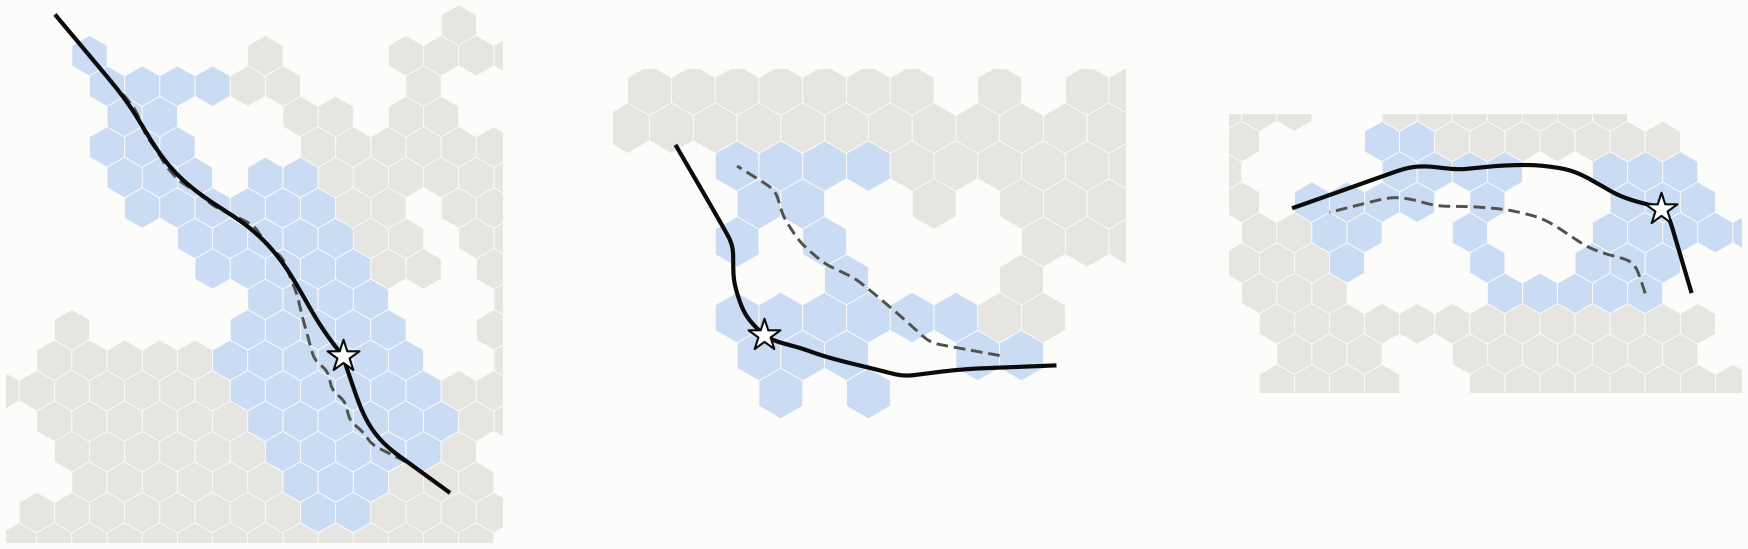
\includegraphics[width=\columnwidth]{bend}
\caption{\textsc{Bend} on three mission clusters: a small offset; a \SI{370}{m} offset (L-shaped cluster); a
\SI{302}{m} offset (U-shaped cluster round a lake). Dashed: smoothed centre curve; solid: final path through the head
(star), with its leads.}
\label{fig:bend}
\end{figure}

\section{Results}
\textbf{Setup.} Geometry: 57 curved domains (\ang{90}, \ang{180} or \ang{270} bends, 0.6 or \SI{1}{km} wide, 4 or 6
clusters' worth of land). Mission: 40 ``lake-block'' maps with $K=2,4,6,8$ clusters (10 each), BS \SI{1}{km} south; the pass and River
run in ns-3 (IEEE 802.15.4 PHY and full MAC~\cite{ieee802154}, urban A2G and G2G channels); the second team is
replayed for 100 random draws per map. Baseline: $k$-medoids clusters flown by \textsc{Chord}.

\begin{figure}[t]
\centering
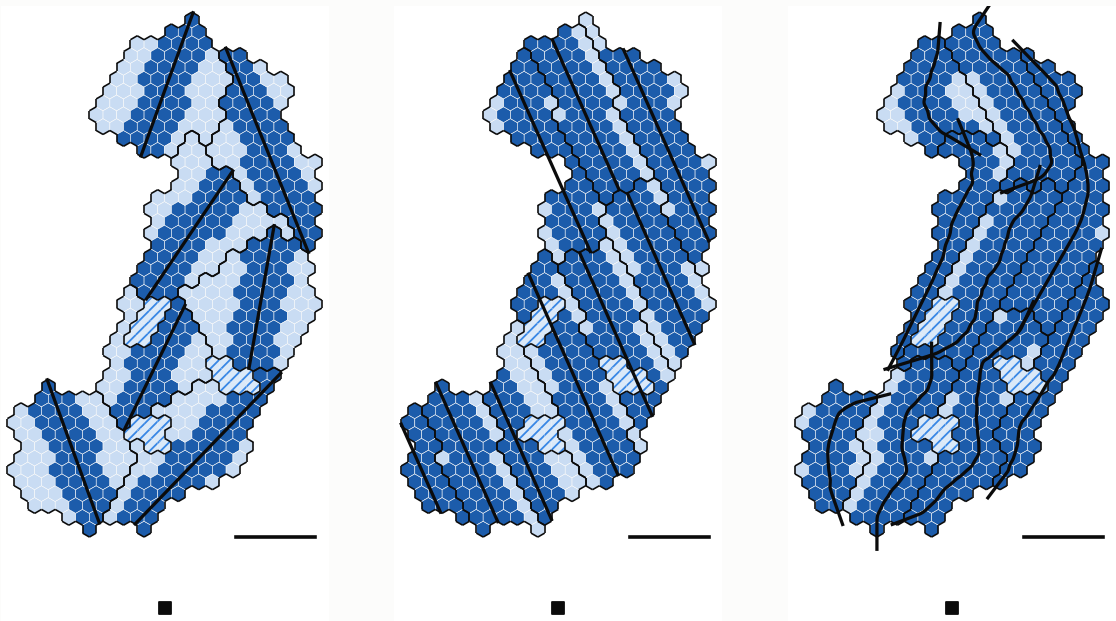
\includegraphics[width=\columnwidth]{compare}
\caption{One curved domain, three partitions: $k$-medoids with \textsc{Chord} (left), straight lanes (middle),
\textsc{Meander} (right). Dark blue: cells within $\omega$ of the own cluster's path; black: paths. River coverage
57, 80 and 88\,\%.}
\label{fig:compare}
\end{figure}

\textbf{Coverage (Table~\ref{tab:geo}, Fig.~\ref{fig:compare}).} Flight-first partitioning puts 83--90\,\% of the
cells within the River band, against 55--57\,\% for $k$-medoids with \textsc{Chord}, and halves the distance of the
farthest cell from its path. On the 40 mission maps it doubles the share of cells that hold all 12 clue images on
their own, without River (17--28\,\% vs.\ 10--14\,\%). Against straight lanes, the geodesic lanes gain most in
narrow bent strips (+8 points at \SI{0.6}{km} and \ang{90}, 10 of 10 domains) and 0--3 points on wide land.

\begin{table}[t]
\caption{Geometry on 57 curved domains (range over six domain classes; distances in cells unless noted)}\label{tab:geo}
\centering\footnotesize
\setlength{\tabcolsep}{3pt}
\begin{tabular}{@{}lccc@{}}
\toprule
 & $k$-med.\ + \textsc{Chord} & Straight lanes & \textsc{Meander}\\
\midrule
Clusters & 5.2--7.8 & 7.2--9.3 & 7.1--9.3\\
River coverage $\varrho$ & 0.55--0.57 & 0.81--0.87 & \textbf{0.83--0.90}\\
Farthest cell from path & 4.8--5.3 & 2.2--2.4 & 2.2--2.8\\
In-cluster flight (km) & 11.0--15.3 & 14.3--20.5 & 17.1--27.1\\
\bottomrule
\end{tabular}
\end{table}

\textbf{Where River saturates (Fig.~\ref{fig:sat}).} We swept strip-shaped clusters of width $W\in\{3,\dots,10\}$
cells and length $L\in\{1.5,\dots,6\}$\,km (75 ns-3 runs). (i)~\emph{Length:} with one \SI{400}{kB} window around the
head, the last critical cell completes 2.7--4.8$\times$ later at \SI{3}{km} than at \SI{2}{km} (53--\SI{102}{s}).
Giving every critical cell the copy of the clue set nearest to it removes this limit: 19--\SI{32}{s} even at
\SI{6}{km}. Below \SI{2}{km} no copy fits. (ii)~\emph{Width:} completion stays at 7--\SI{10}{s} up to about
\SI{600}{m} from the path; the network load per cell grows slowly up to 8 cells (227$\to$385 frames), then
1.6$\times$ at 10 cells and another 2.1$\times$ at 14 cells. (iii)~\emph{Domain level:} the tour dominates, since each
lane fewer saves 100--\SI{150}{s}. The recommended shape is lanes 8--10 cells wide, clusters 2--\SI{3}{km} long
(110--190 cells): $\CapC=80$ is too small for lane clusters.

\begin{figure}[t]
\centering
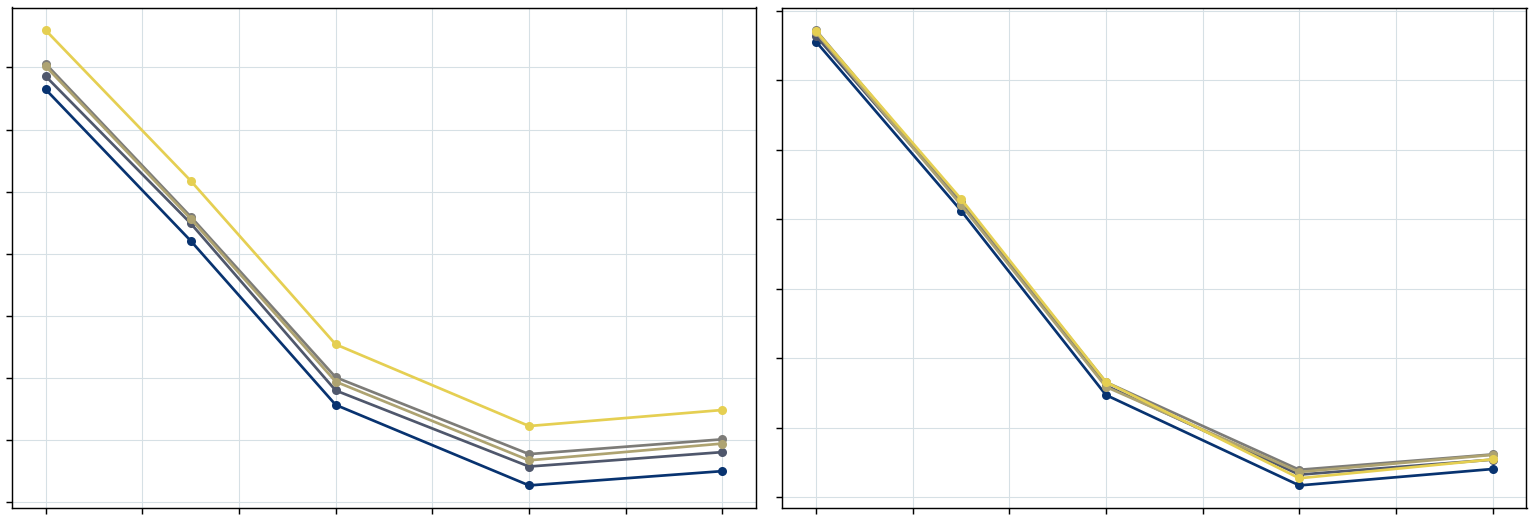
\includegraphics[width=\columnwidth]{sat-domain}
\caption{Domain-level time at which critical cells hold their data on a $6\times\SI{4}{km}$ domain, versus lane width
(3, 4.5, 6, 8, \num{10} cells). Left: mean; right: latest. One line per cluster length, dark blue (\SI{1.5}{km}) to
yellow (\SI{6}{km}). The minimum lies at 8 cells.}
\label{fig:sat}
\end{figure}

\textbf{Mission level (Table~\ref{tab:mission}, Fig.~\ref{fig:diag}).} The coverage gain does not yet turn into a
faster mission. With Dubins links, \textsc{Meander} (tuned: $L=7.5$, $f=\frac12$) finishes 48--\SI{97}{s} later than
$k$-medoids with \textsc{Chord} and wins on at most 2 of 10 maps per size. Three effects explain it:
\begin{itemize}
\item \emph{More clusters} (+20--45\,\% after tuning): more entries, exits and Dubins turns, and more cluster heads,
hence more critical cells for the second team to rank.
\item \emph{Raw data already penetrates.} The A2G link reaches about \SI{1}{km}, so 98--100\,\% of cells hear at
least half of their cluster's data under any partition; River completes the clue set at the critical cells in tens of
seconds.
\item \emph{Same verification once $c^\star$ is known.} With an oracle for $c^\star$ both partitions finish together
(244/287/316/\SI{345}{s} vs.\ 245/287/314/\SI{347}{s}); the loss lies in the longer tour (reports arrive later) and
in the larger candidate set.
\end{itemize}

\begin{table}[t]
\caption{Mission level on 40 maps (Dubins links, 100 draws per map)}\label{tab:mission}
\centering\footnotesize
\setlength{\tabcolsep}{4pt}
\begin{tabular}{@{}llcccc@{}}
\toprule
 & Partition & $K=2$ & $K=4$ & $K=6$ & $K=8$\\
\midrule
Clusters & $k$-med.\ + \textsc{Chord} & 2 & 4 & 6 & 8\\
 & \textsc{Meander} & 3.3 & 6.2 & 9.0 & 12.1\\
 & \textsc{Meander}, tuned & 2.9 & 5.1 & 7.2 & 9.7\\
\midrule
Critical & $k$-med.\ + \textsc{Chord} & 13.5 & 26.9 & 39.9 & 50.1\\
cells & \textsc{Meander} & 16.5 & 30.6 & 47.3 & 59.0\\
 & \textsc{Meander}, tuned & 15.5 & 29.5 & 42.8 & 55.5\\
\midrule
$T^\star$ (s) & $k$-med.\ + \textsc{Chord} & \textbf{420} & \textbf{586} & \textbf{716} & \textbf{824}\\
 & \textsc{Meander} & 487 & 679 & 845 & 987\\
 & \textsc{Meander}, tuned & 479 & 634 & 770 & 921\\
\midrule
Maps won & \textsc{Meander} & 1 & 0 & 0 & 0\\
(of 10) & \textsc{Meander}, tuned & 1 & 1 & 0 & 2\\
\bottomrule
\end{tabular}
\end{table}

\begin{figure}[t]
\centering
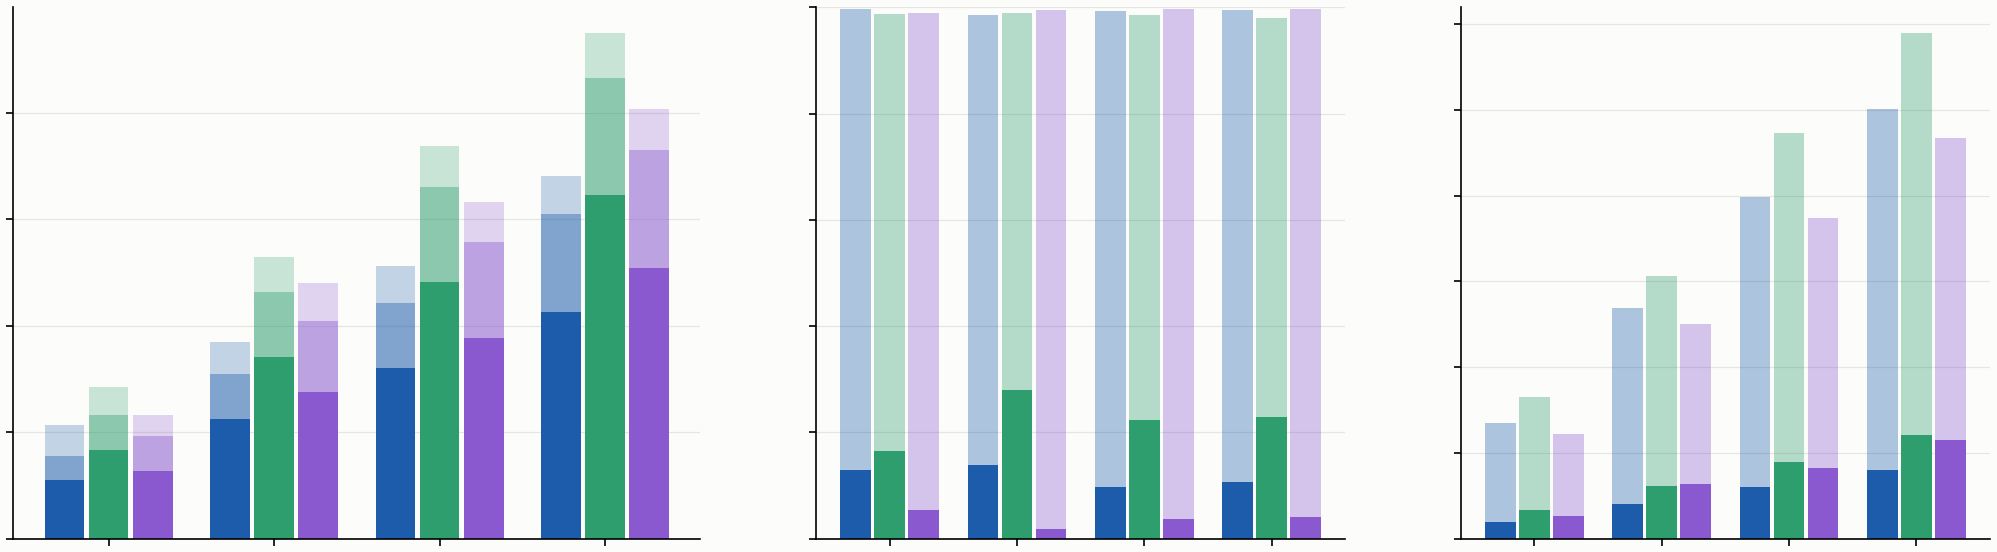
\includegraphics[width=\columnwidth]{diag}
\caption{Diagnosis on the 40 maps, groups $K=2,4,6,8$; bars: $k$-medoids + \textsc{Chord} (blue), \textsc{Meander}
(green), split-cluster baseline (purple). Left: first-team tour, stacked in-cluster (dark), links (medium), return
(light). Middle: cells hearing $\ge50\,\%$ of $D$ (light) and cells holding all 12 clues alone (dark). Right:
critical cells (light) and clusters (dark).}
\label{fig:diag}
\end{figure}

\section{Discussion and Next Steps}
\textbf{What holds.} (i)~Flight geometry is a design variable of the network: \textsc{Chord} alone nearly doubles the
data of a cluster without adding any cluster. (ii)~Geodesic lanes give near-complete River coverage on curved, perforated land with
curvature-feasible paths. (iii)~River's cost depends on the cluster shape in a predictable way, which gives concrete
targets for Layer~2.

\textbf{What does not, yet.} Coverage is not the objective: critical cells need only the clue set, and River supplies
it quickly. Cluster count and tour length dominate $T^\star$. The current \textsc{Meander} also pays costs that do not
belong to the lane idea: lanes cut into fragments by lakes, and a separate path per cluster instead of one continuous
sweep. Kinematics penalise it further, since every cluster boundary is a turn (gap to $k$-medoids
62--\SI{150}{s} with straight links, 67--\SI{163}{s} with Dubins links).

\textbf{Fair comparison (pending).} The partitions above differ in cluster number and size (coefficient of variation
0.16--0.21 vs.\ 0.06--0.11). \textsc{Meander-K} chains all lanes into one boustrophedon sequence that flies over
lakes, cuts it into exactly $K$ equal runs, and keeps the paths, heads and River of \textsc{Meander}; it should be
evaluated at the saturation optimum (lanes about 8 cells) with per-critical-cell windows for both partitions.

\textbf{Use in the ICC paper.} Sections~II--III (model, \textsc{Chord}) fit the system-model part; Section~IV and
Fig.~\ref{fig:steps} can form a ``flight-first clustering'' subsection; Tables~\ref{tab:geo}--\ref{tab:mission} and
Fig.~\ref{fig:sat} support a short Layer-2 evaluation once the fair comparison is run with $N\ge120$.

\bibliographystyle{IEEEtran}
\begin{thebibliography}{9}
\bibitem{dubins1957} L.~E. Dubins, ``On curves of minimal length with a constraint on average curvature, and with
prescribed initial and terminal positions and tangents,'' \emph{Amer. J. Math.}, vol.~79, no.~3, pp.~497--516, 1957.
\bibitem{kaufman1990} L.~Kaufman and P.~J. Rousseeuw, \emph{Finding Groups in Data: An Introduction to Cluster
Analysis}. New York: Wiley, 1990.
\bibitem{heldkarp1962} M.~Held and R.~M. Karp, ``A dynamic programming approach to sequencing problems,'' \emph{J. SIAM},
vol.~10, no.~1, pp.~196--210, 1962.
\bibitem{dijkstra1959} E.~W. Dijkstra, ``A note on two problems in connexion with graphs,'' \emph{Numer. Math.},
vol.~1, pp.~269--271, 1959.
\bibitem{huang2001} W.~H. Huang, ``Optimal line-sweep-based decompositions for coverage algorithms,'' in \emph{Proc.
IEEE ICRA}, 2001, pp.~27--32.
\bibitem{choset2000} H.~Choset, ``Coverage of known spaces: The boustrophedon cellular decomposition,''
\emph{Auton. Robots}, vol.~9, no.~3, pp.~247--253, 2000.
\bibitem{ieee802154} \emph{IEEE Standard for Low-Rate Wireless Networks}, IEEE Std 802.15.4-2020, 2020.
\end{thebibliography}

\end{document}
